\documentclass{beamer}

\usetheme{Boadilla}
\usecolortheme{seagull}

\usepackage{graphics}
\usepackage{tikz}
\usetikzlibrary{%
  positioning,
  decorations.markings,
  decorations.pathmorphing,
  decorations.pathreplacing,
  calc,
  arrows,
  shapes,
  shapes.geometric,
  shapes.arrows,
  patterns,
  fit
}

% Disable beamer navigation symbols
\beamertemplatenavigationsymbolsempty

\title[Towards a more educated guessing]
{Towards a more educated guessing:
Improving ecological forecasts using data constraints}
\author{Alexey Shiklomanov}
\institute{Boston University}
\date{June 4, 2018}

\tikzset{
  majorgrid/.style = {step=1, black, thin},
  minorgrid/.style = {step=0.5, gray, thin},
  tinygrid/.style = {step=0.5, gray!90, very thin},
  pic/.style = {inner sep = 0, outer sep = 0},
  cite/.style = {font = \tiny},
  invisible/.style = {opacity = 0},
  shaded/.style = {opacity = 0.5},
  visible/.style = {opacity = 1},
  ampersand replacement = \&,
  onslide/.code args = {<#1>#2}{\only<#1>{\pgfkeysalso{#2}}},
  show/.style = {invisible, onslide = {#1{visible}}},
  hide/.style = {visible, onslide = {#1{invisible}}}
}
 
% Leaf trait pics
\tikzset {
  trait pic/.style = {inner sep = 3pt, outer sep = 3pt, node distance = 1cm},
  trait label/.style = {above, align = center, inner sep = 5pt, outer sep = 5pt, midway, above, font = \small},
  trait letter/.style = {inner sep = 5pt, outer sep = 4pt, node distance = 0.7cm},
  trait sla/.pic = {
    \node [trait pic] (-SLA 1) {
      \includegraphics[width=16mm]{\string ~/Pictures/common_figures/thinLeaf.png}
    };
    \node [trait pic, inner sep = 5pt] (-SLA 2) [right = of -SLA 1] {
      \includegraphics[height=16mm, angle=90, origin=c]{\string ~/Pictures/common_figures/thickLeaf_magnolia.jpg}
    };
    \draw [<->] (-SLA 1) to node [trait label] {Specific leaf\\area} (-SLA 2);
  },
  trait ll/.pic = {
    \node[trait pic] (-LL 1) {
      \includegraphics[height=16mm, angle=90, origin=c]{\string ~/Pictures/common_figures/pineNeedle.jpg}
    };
    \node[trait pic] (-LL 2) [right = of -LL 1] {
      \includegraphics[width=16mm]{\string ~/Pictures/common_figures/mapleLeaf.jpg}
    };
    \draw [<->] (-LL 1) to node [trait label] {Leaf\\longevity} (-LL 2); 
  },
  trait N/.pic = {
    \node [trait letter] (-N1) {
      \Huge \textbf{\color{blue}N}
    };
    \node [trait letter] (-N2) [right = of -N1] {
      \Huge \textbf{\color{blue!30!white}N}
    };
    \draw [<->] (-N1) to node [trait label] {Leaf N} (-N2);
  },
  trait P/.pic = {
    \node [trait letter] (-P1) {
      \Huge \textbf{\color{red}P}
    };
    \node [trait letter] (-P2) [right = of -P1] {
      \Huge \textbf{\color{red!30!white}P}
    };
    \draw [<->] (-P1) to node [trait label] {Leaf P} (-P2);
  },
  trait Rd/.pic = {
    \node [trait letter] (-Rd1) {
      {\tiny \textbf{CO}$_{2}$}
    };
    \node [trait letter] (-Rd2) [right = of -Rd1] {
      {\Large \textbf{CO}$_{2}$}
    };
    \draw [<->] (-Rd1) to node [trait label] {Dark\\respiration} (-Rd2);
  },
  trait Vcmax/.pic = {
    \node[
    draw, 
    shape = circle,
    outer sep = 5pt,
    decoration = {markings, mark=at position 0.5 with{\arrow{>}}},
    postaction = {decorate}
    ] (-vcmax1) 
    {\tiny Rubisco};
    \node[
    draw,
    very thick,
    shape = circle,
    outer sep = 5pt,
    decoration = {markings, mark=at position 0.5 with{\arrow{>}}},
    postaction = {decorate}
    ] (-vcmax2) [right = of -vcmax1] 
    {\tiny \bf Rubisco};
    \draw [<->] (-vcmax1) to node [trait label] {$V_{c,max}$} (-vcmax2);
  },
  trait Jmax/.pic = {
    \node [trait letter] (-Jmax1) {
      {\tiny $e^-$}
    };
    \node [trait letter] (-Jmax2) [right = of -Jmax1] {
      {\Large $e^-$}
    };
    \draw [<->] (-Jmax1) to node [trait label] {\small $J_{max}$} (-Jmax2);
  }
}

%%% Local Variables:
%%% mode: latex
%%% TeX-master: "main"
%%% End:


\newcommand{\drawgrid}{%
  \draw[tinygrid] (current bounding box.south west) grid (current bounding box.north east);
  \draw[minorgrid] (current bounding box.south west) grid (current bounding box.north east);
  \draw[majorgrid] (current bounding box.south west) grid (current bounding box.north east);
  \fill[red] (0, 0) circle (1mm);
}

\begin{document}

\section{Introduction}

\begin{frame}
  \titlepage
\end{frame}

\begin{frame}
  \makebox[\textwidth]{
    \begin{tikzpicture}

      \node [pic] (thales) {
        \includegraphics[width=3in]{\string ~/Pictures/common_figures/random/thales_of_miletus.jpg}
      };

      \node [anchor = north, align = center] (thales label) at (thales.south)
      {
        Thales of Miletus\\
        The first ecological forecaster \\
        (c.624 - c.546 BC)
      };

    \end{tikzpicture}
  }
\end{frame}

\begin{frame}
  \makebox[\textwidth]{
    \begin{tikzpicture}[
      image/.style = {align=center, outer sep=1pt, inner sep=1pt},
      main image/.style = {image, node distance=5pt},
      small image/.style = {image, node distance=1pt}
      ]
      \newcommand{\hhh}{3cm}
      \newcommand{\ysh}{10mm}

      \node [main image] (forest) {
        \includegraphics[height=\hhh, trim={1cm 0 1cm 0}, clip]{\string ~/Pictures/common_figures/forest_picture.jpg}
      };

      \uncover<2->{
        \node [small image] (carbon) [above left=of forest, yshift=-\ysh] {
          \includegraphics[height=\hhh, trim={3cm 0.5cm 3cm 0.5cm}, clip]{\string ~/Pictures/common_figures/carbon_sequestration.png}
        } edge [<-, bend left] (forest);
      }

      \uncover<3->{
        \node [small image] (bird) [above right=of forest, yshift=-\ysh] {
          \includegraphics[height=\hhh]{\string ~/Pictures/common_figures/endangered_MD_bewicksWren.jpg}
        } edge [<-, bend right] (forest);
      }

      \uncover<4->{
        \node [small image] (tent) [below left = of forest, yshift=\ysh] {
          \includegraphics[height=\hhh, trim={3cm 0 3cm 0}, clip]{\string ~/Pictures/common_figures/shenandoah_camping.jpg}
        } edge [<-, bend left] (forest);
      }

      \uncover<5->{
        \node [small image] (logging) [below right = of forest, yshift=\ysh] {
          \includegraphics[height=\hhh, trim={3cm 0 3cm 0}, clip]{\string ~/Pictures/common_figures/sustainable_logging.jpg}
        } edge [<-, bend right] (forest);
      }
    \end{tikzpicture}
  }
\end{frame}

% TODO: Highlight errors in third reveal
\begin{frame}
  \makebox[\textwidth][c]{
    \begin{tikzpicture}[
      year/.style = {font = \Large}
      ]
      \begin{scope}[show = {<2->}]
        \node[pic] (f2006) {
          \includegraphics[height=45mm]{\string ~/Pictures/common_figures/Friedlingstein_2006_land.jpeg}
        };
        \node[cite, anchor = north] (f2006 cite) at (f2006.south) {
          Friedlingstein et al.\ 2006 \textit{J. Clim.}
        };
        \node[year, anchor = south] (f2006 year) at (f2006.north) {2006};
      \end{scope}
      \begin{scope}[show = {<3->}]
        \node[pic, anchor = west] (f2014) at (f2006.east) {
          \includegraphics[height=45mm]{\string ~/Pictures/common_figures/Friedlingstein2014.png}
        };
        \node[cite, anchor = north] (f2014 cite) at (f2014.south) {
          Friedlingstein et al.\ 2014 \textit{J. Clim.}
        };
        \node[year, anchor = south] (f2014 year) at (f2014.north) {2014};
      \end{scope}
      %\draw<2>[red, ultra thick] ($(figure.east) + (-19mm, 5mm)$) ellipse (1.5cm and 3cm);
      %\drawgrid
    \end{tikzpicture}
  }
\end{frame}

\begin{frame}
  \makebox[\textwidth][c]{
    \begin{tikzpicture}
      \node[pic] (dilbert) {
        \includegraphics[width=120mm]{\string ~/Pictures/common_figures/dilbert_forecasts.png}
      };
      \node[cite, anchor = north east] (dilbert cite) at (dilbert.south east) {
        Dilbert, 12/01/2017
      };
      \node[pic, below = of dilbert, show = {<2->}] (data) {
        Forecasts are guessing plus math \textbf{\textit{plus data}}
      };
    \end{tikzpicture}
  }
\end{frame}

\begin{frame}
  \makebox[\textwidth][c]{
    \begin{tikzpicture}
      \begin{scope}[pic, inner sep = 1mm]
        \matrix (top) {
          \node (satellite) {
            \includegraphics[height=20mm]{\string ~/Pictures/common_figures/landsat_picture.jpg}
          }; \&
          \node (airplane) {
            \includegraphics[height=20mm]{\string ~/Pictures/common_figures/aviris_plane.jpg}
          }; \\
        };
        \matrix[below = 0mm of top] (middle) {
          \node (neon) {
            \includegraphics[height=20mm]{\string ~/Pictures/common_figures/neon_site_design.jpg}
          }; \&
          \node (forestgeo) {
            \includegraphics[height=20mm]{\string ~/Pictures/common_figures/forestgeo_logo.png}
          }; \\
        };
        \matrix[below = 0mm of middle] (bottom) {
          \node (fluxnet) {
            \includegraphics[height=20mm]{\string ~/Pictures/common_figures/fluxnet_logo.jpg}
          }; \&
          \node (trydb) {
            \includegraphics[height=20mm]{\string ~/Pictures/common_figures/trydb_logo.jpg}
          }; \\
        };
      \end{scope}
      \node[below = 2mm of bottom, show = {<2->}] {How to best integrate these data products with models?};
    \end{tikzpicture}
  }
\end{frame}


\begin{frame}<1-4>[label=outline]
  \frametitle{Outline}
  \begin{itemize}
  \item<2-|alert@5> \textit{Leaf traits}
  \item<3-|alert@6> \textit{Leaf spectra}
  \item<4-|alert@7> \textit{Airborne spectroscopy}
  \end{itemize}
\end{frame}

\section{Chapter 1}

\againframe<5>{outline}

\begin{frame}
  \makebox[\textwidth]{
    \begin{tikzpicture}[
      pool/.style = {shape = rectangle, ultra thick},
      flux/.style = {very thick},
      carbon/.style = {flux, black},
      water/.style = {flux, blue}
      ]
      % Tree
      \begin{scope}[show = <1->]
        \fill [brown!70!black] (-0.2, 0) rectangle +(0.4, 3);
        \fill [green!70!black] (0, 3) ellipse (2.5 and 1.7);
        \fill [brown!70] (-4, 0) rectangle (4, -1);
      \end{scope}
      % Fluxes
      \begin{scope}[show = <2->]
        \draw [->, carbon] (-1.4, 4) -- +(0, 2);
        \draw [<-, carbon] (0, 4) -- +(0, 2);
        \node[anchor = east] (respiration) at (-1.4, 5.5) {Respiration};
        \node[anchor = west] (photosynthesis) at (0, 5.5) {Photosynthesis};
      \end{scope}
      % Allocation
      \begin{scope}[show = <3->]
        \path [->, thick] (-0.2, 3.8) edge node {} (-1.7, 2.8);
        \path [->, thick] (0, 3.7) edge node {} (0, 0.85);
      \end{scope}
      \pic[show = <4->] at (3, 4.5) {trait Vcmax};
      \pic[show = <5->] at (3.2, 3) {trait N};
      \pic[show = <6->] at (-4.5, 4) {trait Rd};
      \pic[show = <7->] at (-4.5, 1) {trait sla};
      % \drawgrid
    \end{tikzpicture}
  }
\end{frame}

\begin{frame}<1-3>[label=trymap]
  \makebox[\textwidth]{
    \begin{tikzpicture}[
      map/.style = {anchor = north, outer sep = 1mm}
      ]
      \node[map] (sla map) {
        \includegraphics{\string ~/Documents/job_applications/PNNL_postdoc_Bond-Lamberty/pnnl_jobtalk/figure/map1-1.pdf}
      };
      \node[map, show = {<2->}] (leafn map) at (sla map.south) {
        \includegraphics{\string ~/Documents/job_applications/PNNL_postdoc_Bond-Lamberty/pnnl_jobtalk/figure/map2-1.pdf}
      };
      \node[map, show = {<3->}] (vcmax map) at (leafn map.south) {
        \includegraphics{\string ~/Documents/job_applications/PNNL_postdoc_Bond-Lamberty/pnnl_jobtalk/figure/ma3-1.pdf}
      };
      \node[left = of sla map] (sla lab) {Specific leaf area};
      \node[show = {<2->}] (leafn lab) at (leafn map -| sla lab) {Leaf N content};
      \node[show = {<3->}] (vcmax lab) at (vcmax map -| sla lab) {$V_{c, max}$};
    \end{tikzpicture}
  }
\end{frame}

\begin{frame}
  \frametitle{Trait correlations can provide constraint on unobserved traits.}
  \begin{figure}
    \begin{tikzpicture}[
      image/.style = {anchor = south west, inner sep = 0pt},
      bfill/.style = {draw = none, fill = white}
      ]
      \def\fillrect{(1.7, 1.6) rectangle (7, 5.2)}
      \only<1-2>{%
        \node[image] (X) at (0, 0) {%
          \includegraphics{\string ~/Projects/new-phytologist-traits/np-trait-analysis/figures/multivariate_conceptual/no_covariance_1.png}
        };
      }
      \only<1>{%
        \fill [bfill] \fillrect;
      }
      \only<3>{%
        \node[image] at (0, 0) {%
          \includegraphics{\string ~/Documents/job_applications/nasa_goddard_spectroscopy/jobTalk_beamer/figures/multivariate_conceptual/no_covariance_2.png}
        };
      }
      \only<4>{%
        \node[image] at (0, 0) {%
          \includegraphics{\string ~/Documents/job_applications/nasa_goddard_spectroscopy/jobTalk_beamer/figures/multivariate_conceptual/no_covariance_3.png}
        };
      }
      \only<5-6>{%
        \node[image] (Y) at (0, 0) {%
          \includegraphics{\string ~/Documents/job_applications/nasa_goddard_spectroscopy/jobTalk_beamer/figures/multivariate_conceptual/covariance_1.png}
        };
      }
      \only<5>{
        \fill [bfill] \fillrect;
      }
      \only<7>{%
        \node[image] at (0, 0) {%
          \includegraphics{\string ~/Documents/job_applications/nasa_goddard_spectroscopy/jobTalk_beamer/figures/multivariate_conceptual/covariance_2.png}
        };
      }
      \only<8>{%
        \node[image] at (0, 0) {%
          \includegraphics{\string ~/Documents/job_applications/nasa_goddard_spectroscopy/jobTalk_beamer/figures/multivariate_conceptual/covariance_3.png}
        };
      }
    \end{tikzpicture}
  \end{figure}
\end{frame}

\begin{frame}{The leaf economic spectrum is one well-studied axis of trait covariation.}
  \begin{figure}
    \def\wid{0.35\textwidth}
    \includegraphics[width=\wid]{\string ~/Pictures/common_figures/wright_2004_LES_a_LMA_A_N.png}
    \includegraphics[width=\wid]{\string ~/Pictures/common_figures/wright_2004_LES_b_LL_LMA_R.png}
    \includegraphics[width=\wid]{\string ~/Pictures/common_figures/wright_2004_LES_c_LMA_N_P.png}
  \end{figure}
  {\tiny Wright et al.\ 2004 \textit{Nature}\par}
\end{frame}

\begin{frame}
  \begin{figure}
    \def\wid{60mm}
    \begin{tikzpicture}
      \node[pic] (taiga) {
        \includegraphics[width=\wid]{\string ~/Pictures/common_figures/Taiga_Landscape_in_Canada.jpg}
      };
      \node[pic, right = 2mm of taiga] (savanna) {
        \includegraphics[width=\wid]{\string ~/Pictures/common_figures/African-Savanna-2.jpg}
      };
      \node[pic, below = 2mm of taiga] (desert) {
        \includegraphics[width=\wid]{\string ~/Pictures/common_figures/sonoran-desert.jpg}
      };
      \node[pic, below = 2mm of savanna] (rainforest) {
        \includegraphics[width=\wid]{\string ~/Pictures/common_figures/amazon_rainforest.jpg}
      };
    \end{tikzpicture}
  \end{figure}
\end{frame}

\begin{frame}{How consistent are leaf trait correlations across scales, specifically within and across PFTs?}
  \begin{figure}
    \uncover<2->{\includegraphics[width=0.45\textwidth]{\string ~/Documents/job_applications/nasa_goddard_spectroscopy/jobTalk_beamer/figures/conceptual_groupSame.png}}
    \uncover<3->{\includegraphics[width=0.45\textwidth]{\string ~/Documents/job_applications/nasa_goddard_spectroscopy/jobTalk_beamer/figures/conceptual_groupDiff.png}}
  \end{figure}
  \begin{columns}
    \uncover<4->{
      \begin{column}{0.5\textwidth}
        {\small Fundamental constraint on plant function}
      \end{column}
    }
    \uncover<5->{
      \begin{column}{0.5\textwidth}
        {\small Multiple sources of variability are confounded}
      \end{column}
    }
  \end{columns}
\end{frame}

\begin{frame}{Research questions}
  \begin{figure}
    \begin{tikzpicture}[
      bullet/.style = {align = left, text width = 70mm},
      r1/.style = {invisible, onslide = {<2->{visible}}},
      r2/.style = {invisible, onslide = {<3->{visible}}}
      ]
      \matrix{
        \node[bullet, r1] {1.~How consistent are trait correlations?}; \&
        \node[pic, r1] {\includegraphics[height=35mm]{\string ~/Documents/job_applications/nasa_goddard_spectroscopy/jobTalk_beamer/figures/conceptual_groupDiff.png}}; \\
        \node[bullet, r2] {2.~How useful is multivariate constraint for informing traits?}; \&
        \node[pic, r2] {\includegraphics[height=35mm]{\string ~/Documents/job_applications/nasa_goddard_spectroscopy/jobTalk_beamer/figures/multivariate_conceptual/covariance_3.png}}; \\
      };
    \end{tikzpicture}
  \end{figure}
\end{frame}

\begin{frame}{TRY trait database}
  \begin{figure}
    \includegraphics[width=\textwidth]{\string ~/Documents/job_applications/nasa_goddard_spectroscopy/jobTalk_beamer/figures/data_map.png}
  \end{figure}
\end{frame}

\begin{frame}{7 foliar traits}
  \begin{figure}
    \begin{tikzpicture}[column sep = 5mm]
      \matrix (row 1) {
        \pic {trait ll}; \&
        \pic {trait sla}; \\
      };
      \matrix [anchor = north, yshift = 5mm] (row 2) at (row 1.south) {
        \pic {trait N}; \&
        \pic {trait P}; \\
      };
      \matrix [anchor = north, nodes = {anchor = south}] (row 3) at (row 2.south) {
        \pic {trait Rd}; \&
        \pic {trait Vcmax}; \&
        \pic {trait Jmax}; \\
      };
    \end{tikzpicture}
  \end{figure}
\end{frame}

\begin{frame}{14 plant functional types (PFTs) from the Community Land Model (CLM)}
  \makebox[\textwidth][c]{
    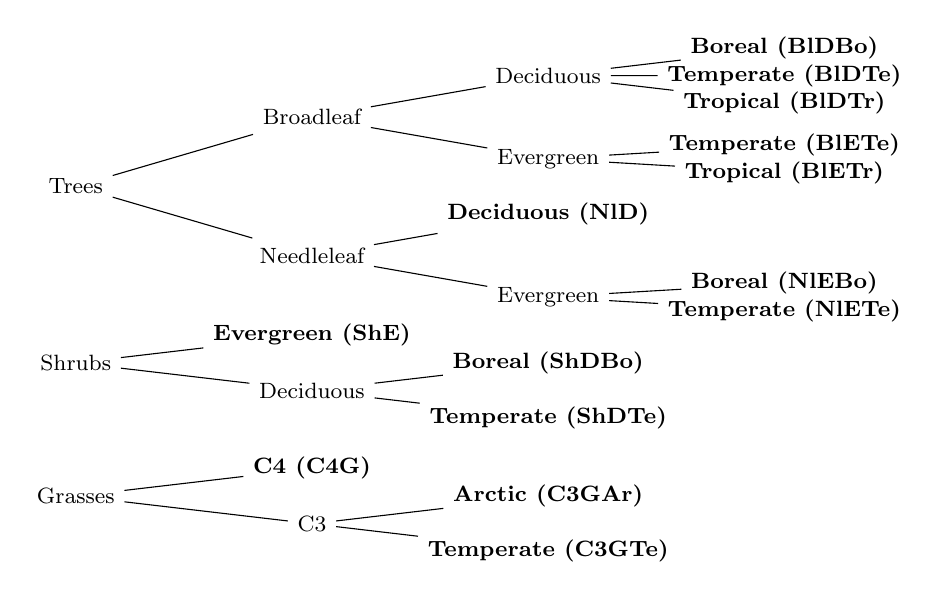
\begin{tikzpicture}[
      grow = right,
      font = \footnotesize,
      level/.style = {level distance = 3cm},
      end/.style = {font = \footnotesize\bf}
      ] 
      \node (trees) {Trees}
        [
        level 1/.style = {level, sibling distance = 5em},
        level 2/.style = {level, sibling distance = 3em},
        level 3/.style = {level, sibling distance = 1em}
        ]
        child {node {Needleleaf}
          child {node {Evergreen}
            child [end] {node {Temperate (NlETe)}}
            child [end] {node {Boreal (NlEBo)}}
          }
          child [end] {node {Deciduous (NlD)}}
        }
        child {node {Broadleaf}
          child {node {Evergreen} 
            child [end] {node {Tropical (BlETr)}}
            child [end] {node {Temperate (BlETe)}}
          }
          child {node {Deciduous}
            child [end] {node {Tropical (BlDTr)}}
            child [end] {node {Temperate (BlDTe)}}
            child [end] {node {Boreal (BlDBo)}}
          }
        }
        ;
      \node (shrubs) [below=1.8cm of trees] {Shrubs}
        [
        level 1/.style = {level, sibling distance = 2em},
        level 2/.style = {level, sibling distance = 2em}
        ]
        child {node {Deciduous}
          child [end] {node {Temperate (ShDTe)}}
          child [end] {node {Boreal (ShDBo)}}
        }
        child [end] {node {Evergreen (ShE)}}
        ;
      \node (grasses) [below=1.25cm of shrubs] {Grasses}
        [
        level 1/.style = {level, sibling distance = 2em},
        level 2/.style = {level, sibling distance = 2em}
        ]
        child {node {C3}
          child [end] {node {Temperate (C3GTe)}}
          child [end] {node {Arctic (C3GAr)}}
        }
        child [end] {node {C4 (C4G)}}
        ;
    \end{tikzpicture}
  }
\end{frame}

\begin{frame}{Multivariate vs.~hierarchical models}
  \begin{columns}[t]
    \uncover<2->{
      \begin{column}{0.5\textwidth}
        \begin{center}
          \textbf{Simple multivariate}
          \begin{figure}
            \includegraphics[width=\textwidth]{\string ~/Documents/job_applications/nasa_goddard_spectroscopy/jobTalk_beamer/figures/conceptual_modelMulti.png}
          \end{figure}
        \end{center}
      \end{column}
    }
    \uncover<3->{
      \begin{column}{0.5\textwidth}
        \begin{center}
          \textbf{Hierarchical}
          \begin{figure}
            \includegraphics[width=\textwidth]{\string ~/Documents/job_applications/nasa_goddard_spectroscopy/jobTalk_beamer/figures/conceptual_modelHier.png}
          \end{figure}
        \end{center}
      \end{column}
    }
  \end{columns}
\end{frame}

\begin{frame}{How consistent are trait correlations across scales?}
  \makebox[\textwidth][c]{
    \begin{tikzpicture}
      \begin{scope}[pic]
        \node [show = {<2>}] (narea sla) {
          \includegraphics{\string ~/Documents/job_applications/PNNL_postdoc_Bond-Lamberty/pnnl_jobtalk/figure/stick_sla_n-1.pdf}
        };
        \node [show = {<3>}] (vcmax jmax) {
          \includegraphics{\string ~/Documents/job_applications/PNNL_postdoc_Bond-Lamberty/pnnl_jobtalk/figure/stick_vcmax_jmax-1.pdf}
        };
        \node [show = {<4>}] (narea ll) {
          \includegraphics{\string ~/Documents/job_applications/PNNL_postdoc_Bond-Lamberty/pnnl_jobtalk/figure/stick_n_ll-1.pdf}
        };
        \node [show = {<5->}] (mainfig) {
          \includegraphics[height=75mm]{\string ~/Projects/new-phytologist-traits/np-trait-analysis/manuscript/_bookdown_files/shiklomanov_newphyt_files/figure-latex/stickpairs-1.pdf}
        };
      \end{scope}
    \end{tikzpicture}
  }
\end{frame}

\begin{frame}{How useful is multivariate constraint for informing trait estimates?}
  \begin{figure}
    \includegraphics[height=0.7\textheight]{\string ~/Projects/new-phytologist-traits/np-trait-analysis/manuscript/_bookdown_files/shiklomanov_newphyt_files/figure-latex/civssamplesize-1.pdf}
  \end{figure}
\end{frame}

\begin{frame}{Takeaways}
  \begin{itemize}
  \item<2-> Leaf economic relationships for all traits except leaf lifespan are
    generally consistent across PFTs
    \item<3-> Multivariate constraint is strong at low sample sizes
    \item<4-> Even with multivariate constraint, many PFTs are severely data limited
  \end{itemize}
  %\begin{figure}
    %\begin{tikzpicture}[
      %bullet/.style = {text width = \textwidth, align = left},
      %b1/.style = {invisible, onslide = {<2->{visible}}},
      %b2/.style = {invisible, onslide = {<3->{visible}}},
      %b3/.style = {invisible, onslide = {<4->{visible}}}
      %]
      %\matrix {
        %\node[bullet, b1] {\textbullet\ Leaf economic relationships for all traits except leaf lifespan are generally consistent across PFTs}; \\
        %\node[bullet, b2] {\textbullet\ Multivariate constraint is strong at low sample sizes}; \\
        %\node[bullet, b3] {\textbullet\ Even with multivariate constraint, many PFTs are severely data limited}; \\
      %};
    %\end{tikzpicture}
  %\end{figure}
\end{frame}

\section{Chapters 2-3}

\againframe<6>{outline}
\againframe<3>{trymap}

\begin{frame}
  \begin{figure}
    \begin{tikzpicture}[
      hl/.style = {very thick, draw = red, shape = circle, radius = 5mm},
      hl line/.style = {very thick, draw = red, ->},
      lab/.style = {anchor = north, font = {\tiny \itshape}}
      ]
      \node[show = {<1>}] {
        \includegraphics{\string ~/Projects/prospect-traits/rspecan/agu_presentation/figure/sla_base-1.pdf}
      };
      \node[show = {<2>}] {
        \includegraphics{\string ~/Projects/prospect-traits/rspecan/agu_presentation/figure/sla2-1.pdf}
      };
      \node[show = {<3>}] {
        \includegraphics{\string ~/Projects/prospect-traits/rspecan/agu_presentation/figure/sla3-1.pdf}
      };
      \node[show = {<4-6>}] {
        \includegraphics{\string ~/Projects/prospect-traits/rspecan/agu_presentation/figure/sla4-1.pdf}
      };

      \node[show = {<7>}] {
        \includegraphics{\string ~/Projects/prospect-traits/rspecan/agu_presentation/figure/sla5-1.pdf}
      };
      \coordinate (d texana) at (5.15, 2.55);
      \coordinate (f grandifolia) at (-3.15, -1.60);
      \coordinate (d texana loc) at (3, 4.1);
      \coordinate (f grandifolia loc) at (-3.9, 4.1);
      \begin{scope}[show = {<5,6>}]
        \node[hl] (d texana hl) at (d texana) {};
        \node[pic, anchor = north east] (d texana pic) at (d texana loc) {
          \includegraphics[width=20mm]{\string ~/Pictures/common_figures/diospyros-texana-leaves.jpg}
        };
        \node[lab] (d texana lab) at (d texana pic.south) {Diospyros texana};
        \draw[hl line] (d texana hl.west) -- (d texana pic.east);
      \end{scope}
      \begin{scope}[show = {<6>}]
        \node[hl] (f grandifolia hl) at (f grandifolia) {};
        \node[pic, anchor = north west] (f grandifolia pic) at (f grandifolia loc) {
          \includegraphics[width=20mm]{\string ~/Pictures/common_figures/fagus-grandifolia-leaves.jpg}
        };
        \node[lab] (f grandifolia lab) at (f grandifolia pic.south) {Fagus grandifolia};
        \draw[hl line] (f grandifolia hl.north) -- (f grandifolia lab.south);
      \end{scope}
    \end{tikzpicture}
  \end{figure}
\end{frame}

\begin{frame}
  \makebox[\textwidth][c]{
    \begin{tikzpicture}[
      quote/.style = {align = left, font = \small \itshape, anchor = north, text width = 70mm}
      ]
      \node[pic] (galadriel) {
        \includegraphics[width=70mm]{\string ~/Pictures/common_figures/Galadriel_at_her_mirror.png}
      };
      \node[quote] (change text) at (galadriel.south) {
        The world has changed. I~feel it in the water. I~feel it in the earth. I~smell it in the air.
      };
      \node[pic, anchor = north west, show = {<3->}] (keeling) at (change text.south) {
        \includegraphics[height=45mm]{\string ~/Pictures/common_figures/keeling_curve.png}
      };
      \node[pic, anchor = east, show = {<2->}] (phenology) at (keeling.west) {
        \includegraphics[height=20mm]{\string ~/Pictures/common_figures/phenology_leaves.jpg}
      };
      \node[pic, below = of keeling, show = {<2>}] {Remote sensing};
    \end{tikzpicture}
  }
\end{frame}

\begin{frame}
  \makebox[\textwidth][c]{
    \begin{tikzpicture}[
      pic/.style = {outer sep = 0.5pt}
      ]
      \node[pic] (leaf) {
        \includegraphics[height=25mm]{\string ~/Pictures/common_figures/fagus-grandifolia-leaves.jpg}
      };
      \node[pic, anchor = west] (fieldspec) at (leaf.east) {
        \includegraphics[height=25mm]{\string ~/Pictures/common_figures/FieldSpec-4-Wide-Res-Pistol.jpg}
      };
      \node[pic, anchor = north west] (aviris plane) at (leaf.south east) {
        \includegraphics[height=20mm]{\string ~/Pictures/common_figures/aviris_plane.jpg}
      };
      \node[pic, anchor = west] (aviris cube) at (aviris plane.east) {
        \includegraphics[width=20mm, angle = 90]{\string ~/Pictures/common_figures/aviris_image_cube.jpeg}
      };
      \node[pic, anchor = north west, xshift = 3mm] (satellite) at (aviris plane.south east) {
        \includegraphics[height=30mm]{\string ~/Pictures/common_figures/landsat_picture.jpg}
      };
      \node (rs text) at (fieldspec.east -| satellite.north) {\Large Remote sensing};
      \draw[thick, green!70!black, show = {<2>}] (leaf.south west) rectangle (fieldspec.north east);
    \end{tikzpicture}
  }
\end{frame}

\begin{frame}
  \begin{figure}
    \begin{tikzpicture}[
      pic/.style = {outer sep = 1pt},
      sig label/.style = {font = \footnotesize, anchor = south}
      ]
      \node[pic, show = {<1-2>}] (spec plot) {
        \includegraphics{\string ~/Projects/prospect-traits/rspecan/agu_presentation/figure/specintro-1.pdf}
      };
      % TODO: Replace Diaz figure with tikz diagrams
      \node[pic, anchor = north, yshift = -7mm, show = {<2>}] (traits) at (spec plot.south) {
        \includegraphics[height=30mm]{\string ~/Pictures/common_figures/diaz_2014_nature_a.png}
      };
      \draw[<->, thick, show = {<2>}] (spec plot) to node[left]{?} node[right]{?} (traits);
      \node[pic, anchor = north, show = {<3>}] (spectra) at (spec plot.north) {
        \includegraphics{\string ~/Projects/prospect-traits/rspecan/agu_presentation/figure/sigspec2-1.pdf}
      };
      \node[pic, anchor = north, show = {<4>}] (rtm) at (spec plot.north) {
        \includegraphics{\string ~/Projects/prospect-traits/rspecan/agu_presentation/figure/rtm1-1.pdf}
      };
    \end{tikzpicture}
  \end{figure}
\end{frame}

\begin{frame}
  \begin{figure}
    \begin{tikzpicture}[remember picture, overlay]
      \node[anchor = north west, yshift = -3mm, xshift = 1mm] (spectra) at (current page.north west) {Spectra};
      \node[right = of spectra, xshift = 3mm] (traits) {Traits}
      edge [<-, thick] node[align = center] {RTM\\inversion} (spectra);
      \node[draw, thick, shape = rectangle, fit = (spectra) (traits)] {};
    \end{tikzpicture}
    \begin{tikzpicture}
      \node[pic, show = {<2->}] (observed) {
        \includegraphics{\string ~/Projects/prospect-traits/rspecan/agu_presentation/figure/observed_spec-1.pdf}
      };
      \begin{scope}[show = {<3->}]
        \node[pic, anchor = north east, yshift = -5mm, xshift = -10mm] (bad fit) at (observed.south) {
          \includegraphics{\string ~/Projects/prospect-traits/rspecan/agu_presentation/figure/bad_fit-1.pdf}
        };
        \node[pic, left = 12mm of observed] (bad bar) {
          \includegraphics{\string ~/Projects/prospect-traits/rspecan/agu_presentation/figure/bad_bar-1.pdf}
        };
        \draw[->, out = 180, in = 90] (observed.west) to (bad fit.north);
      \end{scope}
      \begin{scope}[show = {<4->}]
        \node[pic, anchor = north west, yshift = -5mm, xshift = 10mm] (good fit) at (observed.south) {
          \includegraphics{\string ~/Projects/prospect-traits/rspecan/agu_presentation/figure/good_fit-1.pdf}
        };
        \node[pic, right = 10mm of observed] (good bar) {
          \includegraphics{\string ~/Projects/prospect-traits/rspecan/agu_presentation/figure/good_bar-1.pdf}
        };
        \draw[->, out = 0, in = 90] (observed.east) to (good fit.north);
      \end{scope}
    \end{tikzpicture}
  \end{figure}
\end{frame}

\begin{frame}{Bayesian RTM inversion}
  \begin{figure}
    \begin{tikzpicture}
      \node[pic] (samples) {
      \includegraphics[width=2in]{{\string ~/Projects/prospect-traits/agu_presentation/inversion.Cab}.png}
      };
      \node[pic, anchor = south west, xshift = -3mm] (bad fit) at (samples.north west) {
        \includegraphics[width=1in,height=1in]{\string ~/Projects/prospect-traits/rspecan/agu_presentation/figure/bad_fit-1.pdf}
      };
      \node[pic, anchor = south east, xshift = 3mm] (good fit) at (samples.north east) {
        \includegraphics[width=1in,height=1in]{\string ~/Projects/prospect-traits/rspecan/agu_presentation/figure/good_fit-1.pdf}
      };
      \node[pic, anchor = west, yshift = -6mm, xshift = -3mm, show = {<2->}] (normal dist) at (samples.east) {
        \includegraphics[angle=270]{\string ~/Projects/prospect-traits/rspecan/agu_presentation/figure/normaldist-1.pdf}
      };
      \node[rotate = 90, anchor = south, font = \small] (chl text) at (samples.west) {Chlorophyll $(\mu g ~ cm^{-2})$};
      \node[anchor = north, font = \small] (iter text) at (samples.south) {Iterations};
      \coordinate (bad start) at (-1.5, 1.8);
      \coordinate (good start) at (1, -0.7);
      \draw[->, thick] (bad start) to (bad fit.south);
      \draw[->, thick] (good start) to (good fit.south);
      \node[anchor = west, xshift = 3mm, show = {<2->}, text width = 35mm] at (normal dist.east) {Trait estimate, with uncertainty};
    \end{tikzpicture}
  \end{figure}
\end{frame}

\begin{frame}
  \begin{figure}
    \begin{tikzpicture}
      \node[pic] (data map) {
        \includegraphics[width=\textwidth]{\string ~/Projects/dissertation/draft/3_prospect/figures/data_map.pdf}
      };
    \end{tikzpicture}
  \end{figure}
\end{frame}

\begin{frame}<1-4>[label=questions]{Research questions}
  What can spectra tell us about\ldots
  \begin{enumerate}
  \item<2-|alert@5> \ldots plant stress and physiological responses?
  \item<3-|alert@6> \ldots large-scale drivers of trait variability?
  \item<4-|alert@7> \ldots other traits we can't ``see''?
  \end{enumerate}
\end{frame}

\againframe<5>{questions}

% TODO: Text needs to be bigger
\begin{frame}
  \frametitle{Spectral inversion was able to detect and quantify the effects of\ldots}
  \makebox[\textwidth][c]{
    \begin{tikzpicture}[
      pic label/.style = {anchor = north, align = center}
      ]
      \begin{scope}[show = <2->]
        \node [pic] (shade leaves) at (-3, 2) {
          \includegraphics[width=30mm, angle = -90]{\string ~/Pictures/common_figures/shaded_leaves.jpg}
        };
        \node [pic label] (shade leaves label) at (shade leaves.south) {Sun vs.\ shade};
      \end{scope}
      \begin{scope}[show = <3->]
        \node [pic] (needles) at (2, 2) {
          \includegraphics[width=45mm]{\string ~/Pictures/common_figures/needle_ozone_damage.jpg}
        };
        \node [pic label] (needles label) at (needles.south) {Ozone damage};
      \end{scope}
      \begin{scope}[show = <4->]
        \node [pic] (potato virus) at (-2.8, -2.0) {
          \includegraphics[width=45mm]{\string ~/Pictures/common_figures/potato_virus_y.jpg}
        };
        \node [pic label] at (potato virus.south) {Potato virus Y};
      \end{scope}
      \begin{scope}[show=<5->]
        \node [pic] (soybean) at (2, -1.8) {
          \includegraphics[width=45mm]{\string ~/Pictures/common_figures/soybean_aphid.jpg}
        };
        \node [pic label] (soybean label) at (soybean.south) {Soybean aphid};
      \end{scope}
      \begin{scope}[show = <6->]
        \node [pic] (milkweed) at (6, 0) {
          \includegraphics[width=24mm]{\string ~/Pictures/common_figures/common_milkweed.jpg}
        };
        \node [pic label] (milkweed label) at (milkweed.south) {Drought stress};
      \end{scope}
      \begin{scope}[show = <7->]
        \node [fit = (needles)(needles label), draw = red, ultra thick] {};
        \node [fit = (milkweed)(milkweed label), draw = red, ultra thick] {};
      \end{scope}
    \end{tikzpicture}
  }
\end{frame}

\begin{frame}{Milkweed water stress}
  \begin{figure}
    \begin{tikzpicture}
      \begin{scope}[show = {<2->}]
        \node[pic] (traits plot) {
          \includegraphics{\string ~/Projects/prospect-traits/rspecan/agu_presentation/figure/field_trait_plot-1.pdf}
        };
        \node[anchor = south] (traits lab) at (traits plot.north) {Field traits};
      \end{scope}
      \begin{scope}[show = {<3->}]
        \node[pic, right = of traits plot] (spec plot) {
          \includegraphics{\string ~/Projects/prospect-traits/rspecan/agu_presentation/figure/spec_trait_plot-1.pdf}
        };
        \node[anchor = south] (spec lab) at (spec plot.north) {``Optical'' traits};
      \end{scope}
      \coordinate (water box) at (3.8, -1.8);
      \coordinate (chl box) at (6.4, 2);
      \coordinate (car box) at (3.8, 0.1);
      \begin{scope}[very thick, draw = red, show = {<4->}]
        \foreach \point in {water box, chl box, car box}
        \draw (\point) rectangle +(2.4, 1.8);
      \end{scope}
      \node[pic, show = {<5->}, anchor = south] (milkweed spec) at (spec plot.south) {
        \includegraphics{\string ~/Projects/prospect-traits/rspecan/agu_presentation/figure/milkweed_spec_plot-1.pdf}
      };
    \end{tikzpicture}
  \end{figure}
\end{frame}

\begin{frame}{Needle damage}
  \begin{figure}
    \begin{tikzpicture}
      \node[pic] (damage) at (0, 0) {
        \includegraphics[width=50mm]{\string ~/Pictures/common_figures/needle_ozone_damage.jpg}
      };
      \node[align = left, anchor = north, font = \small] at (damage.south) {
        H - Healthy\\
        WF - Winter Fleck\\
        CM - Ozone damage
      };
      \node[pic, anchor = west] (needle plot) at ([xshift=5mm] damage.east) {
        \includegraphics{\string ~/Projects/prospect-traits/rspecan/agu_presentation/figure/needle_plot-1.pdf}
      };
      \node[pic, anchor = north] (needle legend) at (needle plot.south) {
        \includegraphics{\string ~/Projects/prospect-traits/rspecan/agu_presentation/figure/needle_legend-1.pdf}
      };
    \end{tikzpicture}
  \end{figure}
\end{frame}

\againframe<6>{questions}

\begin{frame}
  \frametitle{Optical traits vary almost as much within as across species.}
  \begin{figure}
    \centering
    \includegraphics[height=3in]{\string ~/Projects/dissertation/draft/3_prospect/figures/within_vs_across.pdf}
  \end{figure}
\end{frame}

\begin{frame}
  \frametitle{Optical trait variability across species is idiosyncratic.}
  \begin{figure}
    \centering
    \includegraphics[height=3in]{\string ~/Projects/dissertation/draft/3_prospect/figures/across_species_anova.pdf}
  \end{figure}
\end{frame}

\againframe<7>{questions}

\begin{frame}
  \makebox[\textwidth][c]{
    \begin{tikzpicture}[my text/.style = {align = center, text width = 125mm, font = \footnotesize}]
      \node [pic] (ridgeplot) {
        \includegraphics[height=3in]{\string ~/Projects/prospect-traits/rspecan/manuscript/figures/zpres_correlation_ridge.pdf}    
      };
      \node [anchor = south, my text, show = <2->] at (ridgeplot.north) {
        Within-species correlations of optical traits with other traits
        are \textbf{species-specific}\ldots
      };
      \node [anchor = north, my text, show = <3->] at (ridgeplot.south) {
        \ldots but tend to be stronger for {\color{red} broadleaved}
        and {\color{green!40!black} needleleaved} trees than
        {\color{cyan!80!black} grasses} and {\color{violet} herbs}.
      };
    \end{tikzpicture}
  }
\end{frame}

\begin{frame}
  \makebox[\textwidth][c]{
    \begin{tikzpicture}[
      my text/.style = {text width = 120mm},
      my label/.style = {font = \small}
      ]
      \node [pic] (corrplot) {
        \includegraphics[height=3in, trim = {20mm 20mm 0 15mm}, clip]{\string ~/Projects/prospect-traits/rspecan/manuscript/figures/zpres_trait_correlations_species.pdf}
      };
      \node [my label] at (corrplot.north) {Optical trait};
      \node [my label, rotate = 90] at (corrplot.west) {Other trait}; 
      \node [my label, rotate = -90] at ([xshift = 3mm] corrplot.east) {Across-species correlation coefficient};
      \coordinate (meso tl) at (-2.9, 3.7);
      \coordinate (lma tl) at (2.3, 3.7);
      \coordinate (chl tl) at (-1.8, 3.7);
      \begin{scope}[show = <2->]
        \node [my text, anchor = north] at (corrplot.south) {
          {\color{red} Structural} traits are less plastic than
          {\color{blue} functional} traits,
          and therefore have weaker across-species correlations than
          photosynthetic traits.
        };
        \draw [red, ultra thick] (meso tl) rectangle +(0.9, -7.4);
        \draw [red, ultra thick] (lma tl) rectangle +(0.9, -7.4);
      \end{scope}
      \draw [blue, ultra thick, show = <3->] (chl tl) rectangle +(4.0, -7.4);
    \end{tikzpicture}
  }
\end{frame}

\begin{frame}{Takeaways}
  \begin{itemize}
  \item<2-> Spectra can detect stress, and give us hints about its causes.
  \item<3-> Inter- and intra-specific trait variability are comparable, and interspecific variability is idiosyncratic.
  \item<4-> Optical traits are often, but far from always, correlated with other traits.
  \end{itemize}
\end{frame}

\section{Chapter 4}

\againframe<7>{outline}

\begin{frame}
  \begin{figure}
    \centering
    \includegraphics[height=3in]{\string ~/Pictures/common_figures/Friedlingstein2014.png}
  \end{figure}
\end{frame}

\begin{frame}
  \makebox[\textwidth]{
    \begin{tikzpicture}
      \node [pic] (rtm) at (-3, 4.2) {
        \includegraphics[height=1.6in]{\string ~/Pictures/common_figures/fisher_2017_rtm.jpg}
      };
      \node [align = center] at ([xshift=2cm] rtm.east) (rtm text) {Competition\\for light};
      \node [pic, xshift = 20mm] at (0, 0) (water) {
        \includegraphics[height=1.6in, clip, trim = {0 6cm 0 0}]{\string ~/Pictures/common_figures/fisher_2017_water.jpg}
      };
      \node [align = center] at ([xshift=-3.5cm] water.west) (water text) {Competition for water};
      \node [fit = (rtm)(rtm text), draw = red, thick, show = <2->] {};
    \end{tikzpicture}
  }
  % Two points:
  % (1) Models represent processes differently
  % (2) At some point, models become abstractions of reality. No real-life "traits" to measure.
\end{frame}

\begin{frame}
  \makebox[\textwidth][c]{
    \begin{tikzpicture}
      \node [pic] (cycle) {
        \includegraphics[height=3.2in, trim = {0 0 45mm 0}, clip]{\string ~/Pictures/common_figures/dietze_forcast_cycle.jpg}
      };
    \end{tikzpicture}
  }
\end{frame}

\begin{frame}
  \makebox[\textwidth]{%
    \begin{tikzpicture}[
      arrow/.style = {->, line width = 0.4mm},
      image/.style = {align = center, outer sep = 1pt, inner sep = 1pt},
      top image/.style = {image, anchor = north},
      arrow/.style = {->, line width = 0.4mm},
      pic label/.style = {anchor = south, font = \scriptsize}
      ]
      \coordinate (box top) at (0, 5);
      \node [top image] (ed) at ([xshift=-3.5cm] box top) {
        \includegraphics[height=4cm]{\string ~/Pictures/common_figures/ED2_colored.png}
      };
      \node [pic label] (ed label) at (ed.north) {Ecosystem Demography (ED2) Model};
      \draw [thick, red, show = <2->] (-5.1, 2.2) rectangle (-2.1, 3.7);

      \begin{scope}[show = <3->]
        \node [image, anchor = north west] (prospect) at ([xshift=14mm] ed.north east) {
          \includegraphics[height=4cm]{\string ~/Documents/job_applications/PNNL_postdoc_Bond-Lamberty/pnnl_jobtalk/figure/rtm1-1.pdf}
        };
        \node [pic label] (prospect label) at (prospect.north) {PROSPECT leaf RTM};
        \coordinate (plus) at ($(ed.east) !0.5! (prospect.west)$);
        \node [font = \Huge] at (plus) {+};
      \end{scope}

      \begin{scope}[show = <4->]
        \node [font = \Huge, anchor = west] at (prospect.east) {=};
        \node [top image] (aviris sim) at (-2.5, 0.3) {
          \includegraphics[height=4cm]{\string ~/Projects/nasa-rtm/nasa_ef_2018/figures/edr_simple_simulations.png}
        };
        \node [pic label] at (aviris sim.north) {Simulated surface reflectance};
        \node [font = \Huge, anchor = east] at (aviris sim.west) {=};
      \end{scope}

      \begin{scope}[show = <5->]
        \node [top image] (landsat sim) at (3, 0.3) {
          \includegraphics[height=4cm]{\string ~/Projects/nasa-rtm/nasa_ef_2018/figures/edr_simulations_landsat.png}
        };
        \node [pic label] at (landsat sim.north) {Simulated Landsat observations};
        \draw [arrow] (aviris sim.east) -- (landsat sim.west);
      \end{scope}

    \end{tikzpicture}
  }
\end{frame}

\begin{frame}
  \begin{figure}
    \centering
    \includegraphics[height=\textheight]{\string ~/Projects/dissertation/draft/4_edr/figures/sites_both.pdf}
  \end{figure}
\end{frame}

\begin{frame}<1-3>[label = ch4_questions] \frametitle{Research questions}
  \begin{itemize}
  \item<2-|alert@4> How realistic is the representation of canopy radiative transfer in ED2?
  \item<3-|alert@5> Where the model is wrong, how can it be fixed?
  \end{itemize}
\end{frame}

\againframe<4>{ch4_questions}

% Some sites, we nail the spectra and the LAI...
\begin{frame}
  \makebox[\textwidth][c]{
    \begin{tikzpicture}
      \node [pic] (figure) at (0, 0) {
        \includegraphics[width=4in]{\string ~/Projects/nasa-rtm/edr-da/figures/presentation/good_sites.pdf}
      };
      \node [align = center, anchor = south] (title) at (figure.north) {
        At some sites, model reproduces spectra and LAI well.
      };
    \end{tikzpicture}
  }
\end{frame}

% Some sites, we nail the spectra, but with the wrong LAI.
% Problems with identifiability of structure parameters.
\begin{frame}
  \makebox[\textwidth][c]{
    \begin{tikzpicture}
      \node[pic] (figure) at (0, 0) {
        \includegraphics[width=4in]{\string ~/Projects/nasa-rtm/edr-da/figures/presentation/bad_lai.pdf}
      };
      \node [align = center, anchor = south] (title) at (figure.north) {
        At some sites, model reproduces spectra, but with the wrong LAI\ldots
      };
    \end{tikzpicture}
  }
\end{frame}

% Some sites, we get the LAI right, but the spectra wrong.
% Here, because clumping factor. 
% PFT-specific structure parameters are too coarse
% Need a more dynamic representation of structure.
\begin{frame}
  \makebox[\textwidth][c]{
    \begin{tikzpicture}
      \node[pic] (figure) at (0, 0) {
        \includegraphics[width=4in]{\string ~/Projects/nasa-rtm/edr-da/figures/presentation/sites_lh.pdf}
      };
      \node [align = center, anchor = south] (title) at (figure.north) {
        \ldots and at others, model reproduces LAI, but not spectra.
      };
    \end{tikzpicture}
  }
\end{frame}

\begin{frame}{\textbf{Future direction}: Using remote sensing time series to evaluate model dynamics}
  \begin{figure}
    \centering
    \includegraphics[height=3in]{\string ~/Projects/nasa-rtm/edr-da/figures/presentation/landsat_ts_sub.pdf}
  \end{figure}
\end{frame}

\begin{frame} \frametitle{Takeaways}
  \begin{itemize}
  \item ED2 radiative transfer has several problems\ldots
    \begin{itemize}
    \item Wood reflectance is wrong
    \item Ill-posedness of structural parameters
    \item Excessive sensitivity to soil background
    \end{itemize}
  \item \ldots but comparison against remote sensing data is a promising approach.
  \end{itemize}
\end{frame}

\section{Conclusions}

\begin{frame} \frametitle{Conclusions}
  Modeling is hard.
\end{frame}

\end{document}

%%% Local Variables:
%%% mode: latex
%%% TeX-master: t
%%% truncate-lines: 1
%%% truncate-partial-width-windows: nil
%%% End:
